\documentclass[a4paper]{article}
\usepackage{graphicx}
\graphicspath{{img/}}

\title{Cloud Computing Paper Reading Report}
\author{Jianzhong LI 13354146, Tong XU 13354146, Zhengyuan WEI 13354146}

\begin{document}
    \maketitle
    \section{Semantic Home Photo Categorization}
        \subsection{Basic Idea}
        This paper proposed a semantic categorization method for generic home photo, which exploit a two-layered classification model detecting the local and global photo semantics in a feed-forward way. The scheme of two-layered categorization is as follows:

        \begin{figure}[!htb] \begin{center}
             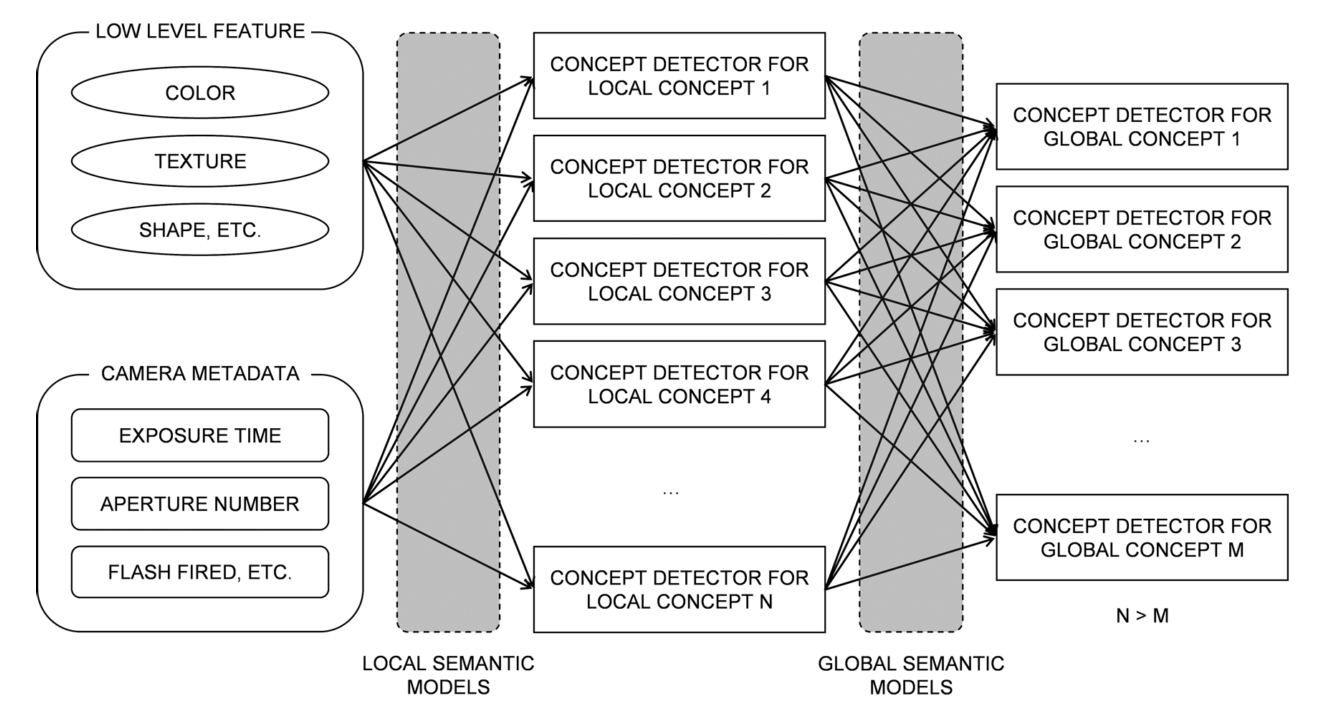
\includegraphics[scale=0.3]{scheme}
             \caption{Two-layered categorization scheme}
        \end{center} \end{figure}

        The overall procedure of the proposed home photo categorization is:
        \begin{enumerate}
            \item A photo input
            \item Camera metadata extraction
            \item Regional division for local photo semantics
            \item Low-level feature extraction
            \item Combination of camera metadata and low-level features
            \item Local semantic classification
            \item New feature generation by concept merging
            \item Global semantic classification
        \end{enumerate}

        \subsection{Motivation}
        Thanks to the development of technology, mobile phones equiped with cameras and other digital devices for capturing photos and videos are ubiquitous. The need for semantic categorization has been raised in managing personal photo albums. Up to the time this paper was published, multilabel detection problem with camera metadata is missing. Therefore, a new semantic categorization was proposed in this paper.
        \subsection{Contribution}
        This paper exploits a novel multilayered classification model that combines camera metadata, low-level features, and intermediate level of semantic features, especially for multilabel classification. The proposed two-layered scheme reduces the error accumulation in many probability models.
        \subsection{Comment}
        According to the paper, the proposed two-layered SVM performed better to classify visual semantics for general home photos, comparing to a major conventional method modeled by a Bayesian network. However, the performance of the model proposed in this paper is still not very satisfying in practice. Other syntactic features, like keyword, spatial context, user annotations are not considered in this paper, either.
        

    \section{User-Friendly Personal Photo Browsing for Mobile Devices}
        \subsection{Basic Idea}
        This paper proposed a user-friendly mobile photo album system, which enable users to browse their photos along semantically meaningful axes of events, personal identities, and categories with minimum maual effort. The hierachy of semantic albuming concepts is as follows.

        \begin{figure}[!htb] \begin{center}
             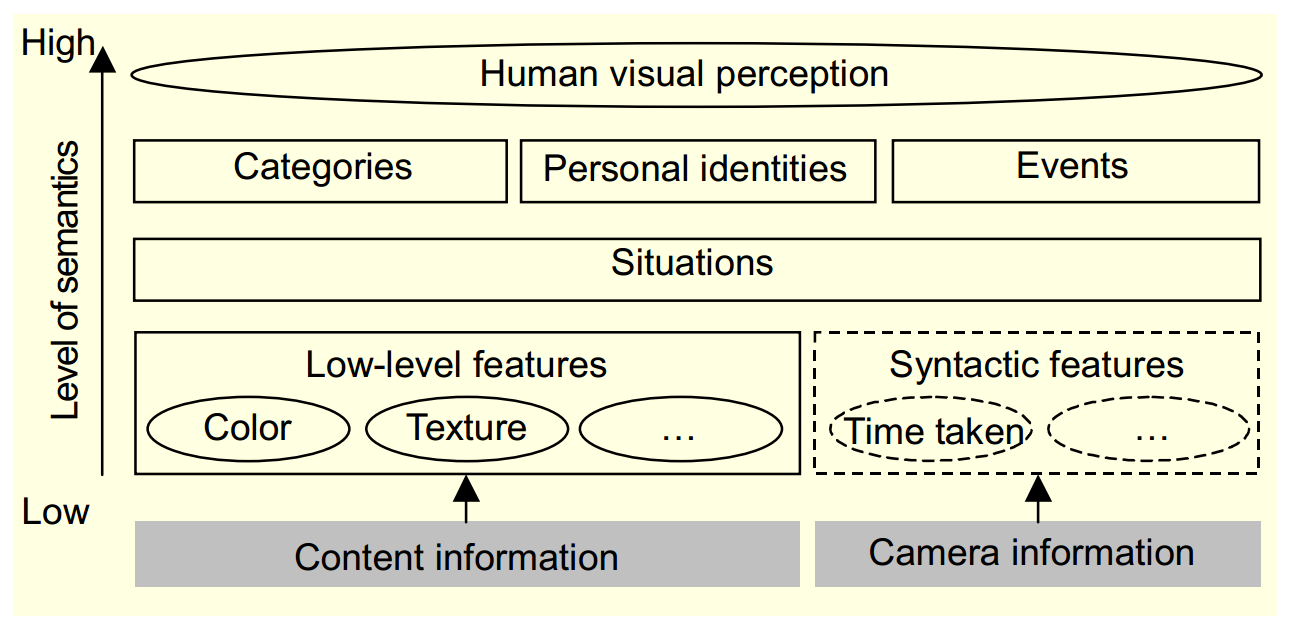
\includegraphics[scale=0.3]{hierachy}
             \caption{Hierarchy of semantic albuming concepts.}
        \end{center} \end{figure}

        The target concepts(events, categories, and personal identities) are close to human visual perception. Basically, content-based low-level features are combined into syntatic features in order to obtain the target concepts.

        \subsection{Motivation}
        Mobile phones equipped with digital cameras and other digital devices for capturing photos and videos are ubiquitous nowadays. People would like to categorize their photos into ``albums". The main problem with the traditional digital photo album is that users usually have to do almost all the job manually, which is time-consuming, tedious, error-prone and inconsistent. Some automatic or semi-automatic mehtods are strongly required to manage such greate number of photos.

        \subsection{Contribution}
        Defining the concept of a meaningful group is one of the most difficult problems to resolve, as people often have different preferences or tendencies regarding how to classify thier photos. This paper proposed three albuming functions, including event-based photo clustering, category-based photo classification and face-based photo search and retrieval. Those functions are light enough to be successfully processed in a mobile computing environment.

        \subsection{Comment}
        Photo categorization is useful in many senarios. But it's also difficult as people often have different preference or tendencies regarding how to classify their photos. Referring to its references, this paper is actually an application (with some improvement) of all those concepts and methods proposed by other scholars.

        The biggest drawback of the system is that the model training for the categories and faces/eyes has to be performed on an off-line PC, which makes this system unrealistic. Inspired by the hierachy of semantic albuming concepts, our team propose a cloud-based user-friendly photo albuming android app. The training can be done on the cloud and the data will be directly download through the mobile Internet.

    \section{Big Data computing and clouds: Trends and future directions}
        \subsection{Basic Idea} 
        This paper discuss approaches and environments for analytics of Big Data on Clouds, which revolves four important areas, including (i) data management and supporting architectures; (ii) model development and assessment; (ii) visualisation and user interaction; and (iv) business models. Open challenges and possible gaps are also covered and recommendations are provided for the research community on future directions on Cloud-support Big Data Computing and analytics solutions.
        \subsection{Motivation}
        Although Cloud computing offers elastic capacity to supply computational resources on demand, the area is still in its early days. Plenty of algorithms and models are proposed, which could be a chellenge for beiginners who have just stepped in this area. Reviews like this paper are needed to provide methodology, recommendations on future directions.
        \subsection{Contribution}
        This paper introduces the key stages of Big Data analytics workflows, and surveyed the state-of-art of each stage in the context of Cloud computing. Surveyed work was classified into three key groups:
        \begin{itemize}
            \item Data Management
            \item Model Building and Scoring
            \item Visualisation and User Interaction. 
        \end{itemize}
        For each areas, ongoing work was analysed and open challenges were discussed.
        \subsection{Comment}
        Plenty of solution for Big Data analytics on Cloud have been created to fit the wide range of analytics requirements. But they may, sometimes, overwhelm non-experienced beginners, like myself. Noted that security is considered an extensive topic, and is not discussed in this paper.
        
\end{document}